%%\documentclass[a4paper, 12pt]{scrreprt}

\documentclass[a4paper, 12pt]{scrartcl}
%usepackage[german]{babel}
\usepackage{microtype}
%\usepackage{amsmath}
%usepackage{color}
\usepackage[utf8]{inputenc}
\usepackage[T1]{fontenc}
\usepackage{wrapfig}
\usepackage{lipsum}% Dummy-Text
\usepackage{multicol}
\usepackage{alltt}
%%%%%%%%%%%%bis hierhin alle nötigen userpackage
\usepackage{tabularx}
\usepackage[utf8]{inputenc}
\usepackage{amsmath}
\usepackage{amsfonts}
\usepackage{amssymb}

%\usepackage{wrapfig}
\usepackage[ngerman]{babel}
\usepackage[left=25mm,top=25mm,right=25mm,bottom=25mm]{geometry}
%\usepackage{floatrow}
\setlength{\parindent}{0em}
\usepackage[font=footnotesize,labelfont=bf]{caption}
\numberwithin{figure}{section}
\numberwithin{table}{section}
\usepackage{subcaption}
\usepackage{float}
\usepackage{url}
%\usepackage{fancyhdr}
\usepackage{array}
\usepackage{geometry}
%\usepackage[nottoc,numbib]{tocbibind}
\usepackage[pdfpagelabels=true]{hyperref}
\usepackage[font=footnotesize,labelfont=bf]{caption}
\usepackage[T1]{fontenc}
\usepackage {palatino}
%\usepackage[numbers,super]{natbib}
%\usepackage{textcomp}
\usepackage[version=4]{mhchem}
\usepackage{subcaption}
\captionsetup{format=plain}
\usepackage[nomessages]{fp}
\usepackage{siunitx}
\sisetup{exponent-product = \cdot, output-product = \cdot}
\usepackage{hyperref}
\usepackage{longtable}
\newcolumntype{L}[1]{>{\raggedright\arraybackslash}p{#1}} % linksbündig mit Breitenangabe
\newcolumntype{C}[1]{>{\centering\arraybackslash}p{#1}} % zentriert mit Breitenangabe
\newcolumntype{R}[1]{>{\raggedleft\arraybackslash}p{#1}} % rechtsbündig mit Breitenangabe
\usepackage{booktabs}
\renewcommand*{\doublerulesep}{1ex}
\usepackage{graphicx}
\usepackage{chemformula}


\usepackage[backend=bibtex, style=chem-angew, backref=none, backrefstyle=all+]{biblatex}
\bibliography{Literatur.bib}
\defbibheading{head}{\section{Literatur}\label{sec:Lit}} 
\let\cite=\supercite
%\begin{document}
%\setlength\abovedisplayshortskip{20pt}
%\setlength\belowdisplayshortskip{20pt}
%\setlength\abovedisplayskip{20pt}
%\setlength\belowdisplayskip{20pt}
\section {Auswertung}
Die exakte Spaltbreite wurde ermittelt indem die Beugung eines Lasers bekannter Wellenlänge bei unterschiedlichen Spaltbreiten gemessen wurde. Es wurde mit Igor Pro ein Querschnitt der Beugungsmusterbestimmt. Die so erhaltenen Intensitätsprofile wurden mit einer, vom Assistenten zur Verfügung gestellten Fitfunktion angepasst. Exemplarisch sind hier das Beugungsmuster\ref{HeNe_0} und das Profil \ref{HeNe_0_Prof} für die Spalteinstellung $0$ gezeigt.

\begin{figure}[H]
	\centering	
	\begin{minipage}{1\textwidth}
		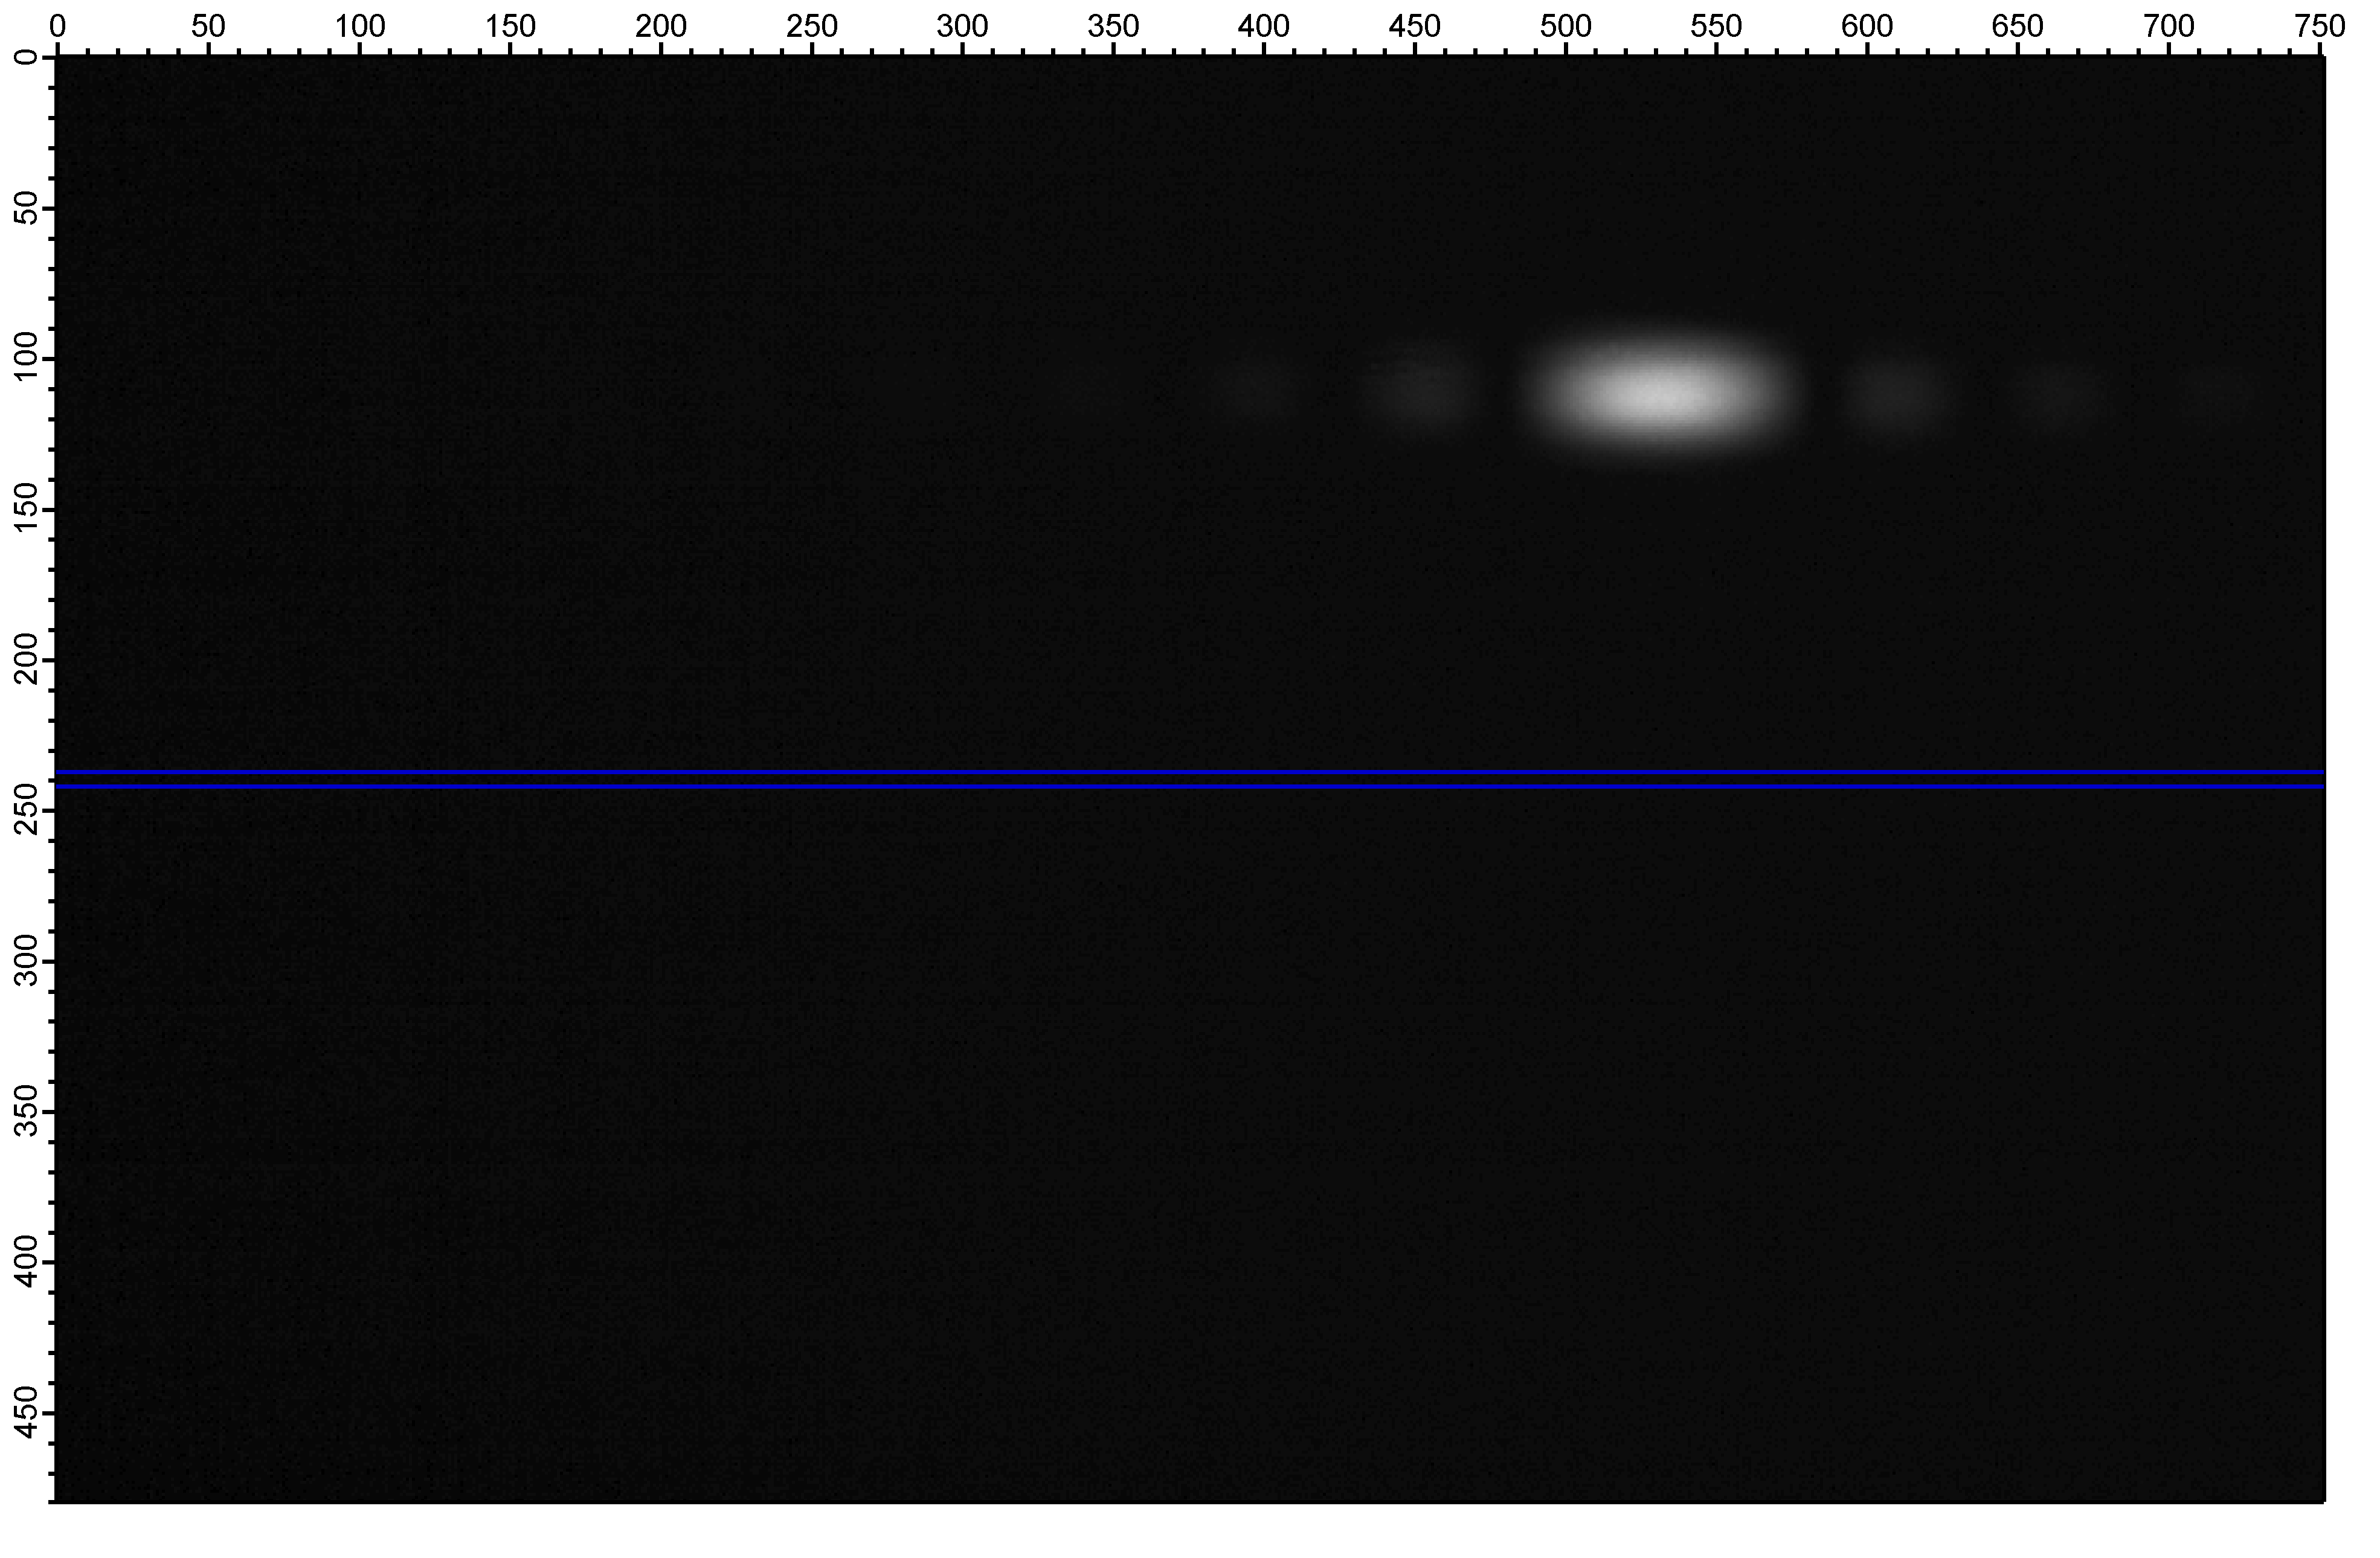
\includegraphics[width=\columnwidth]{180618/Graph0.png}
	\end{minipage}
	\caption{Beugungsmuster eines Helium-Neon-Lasers bei der Einstellung von $0$. Der Querschnitt wurde mit Igor Pro ausgewählt und weiter analysiert }
	\label{HeNe_0}
\end{figure}

\begin{figure}[H]
	\centering	
	\begin{minipage}{1\textwidth}
		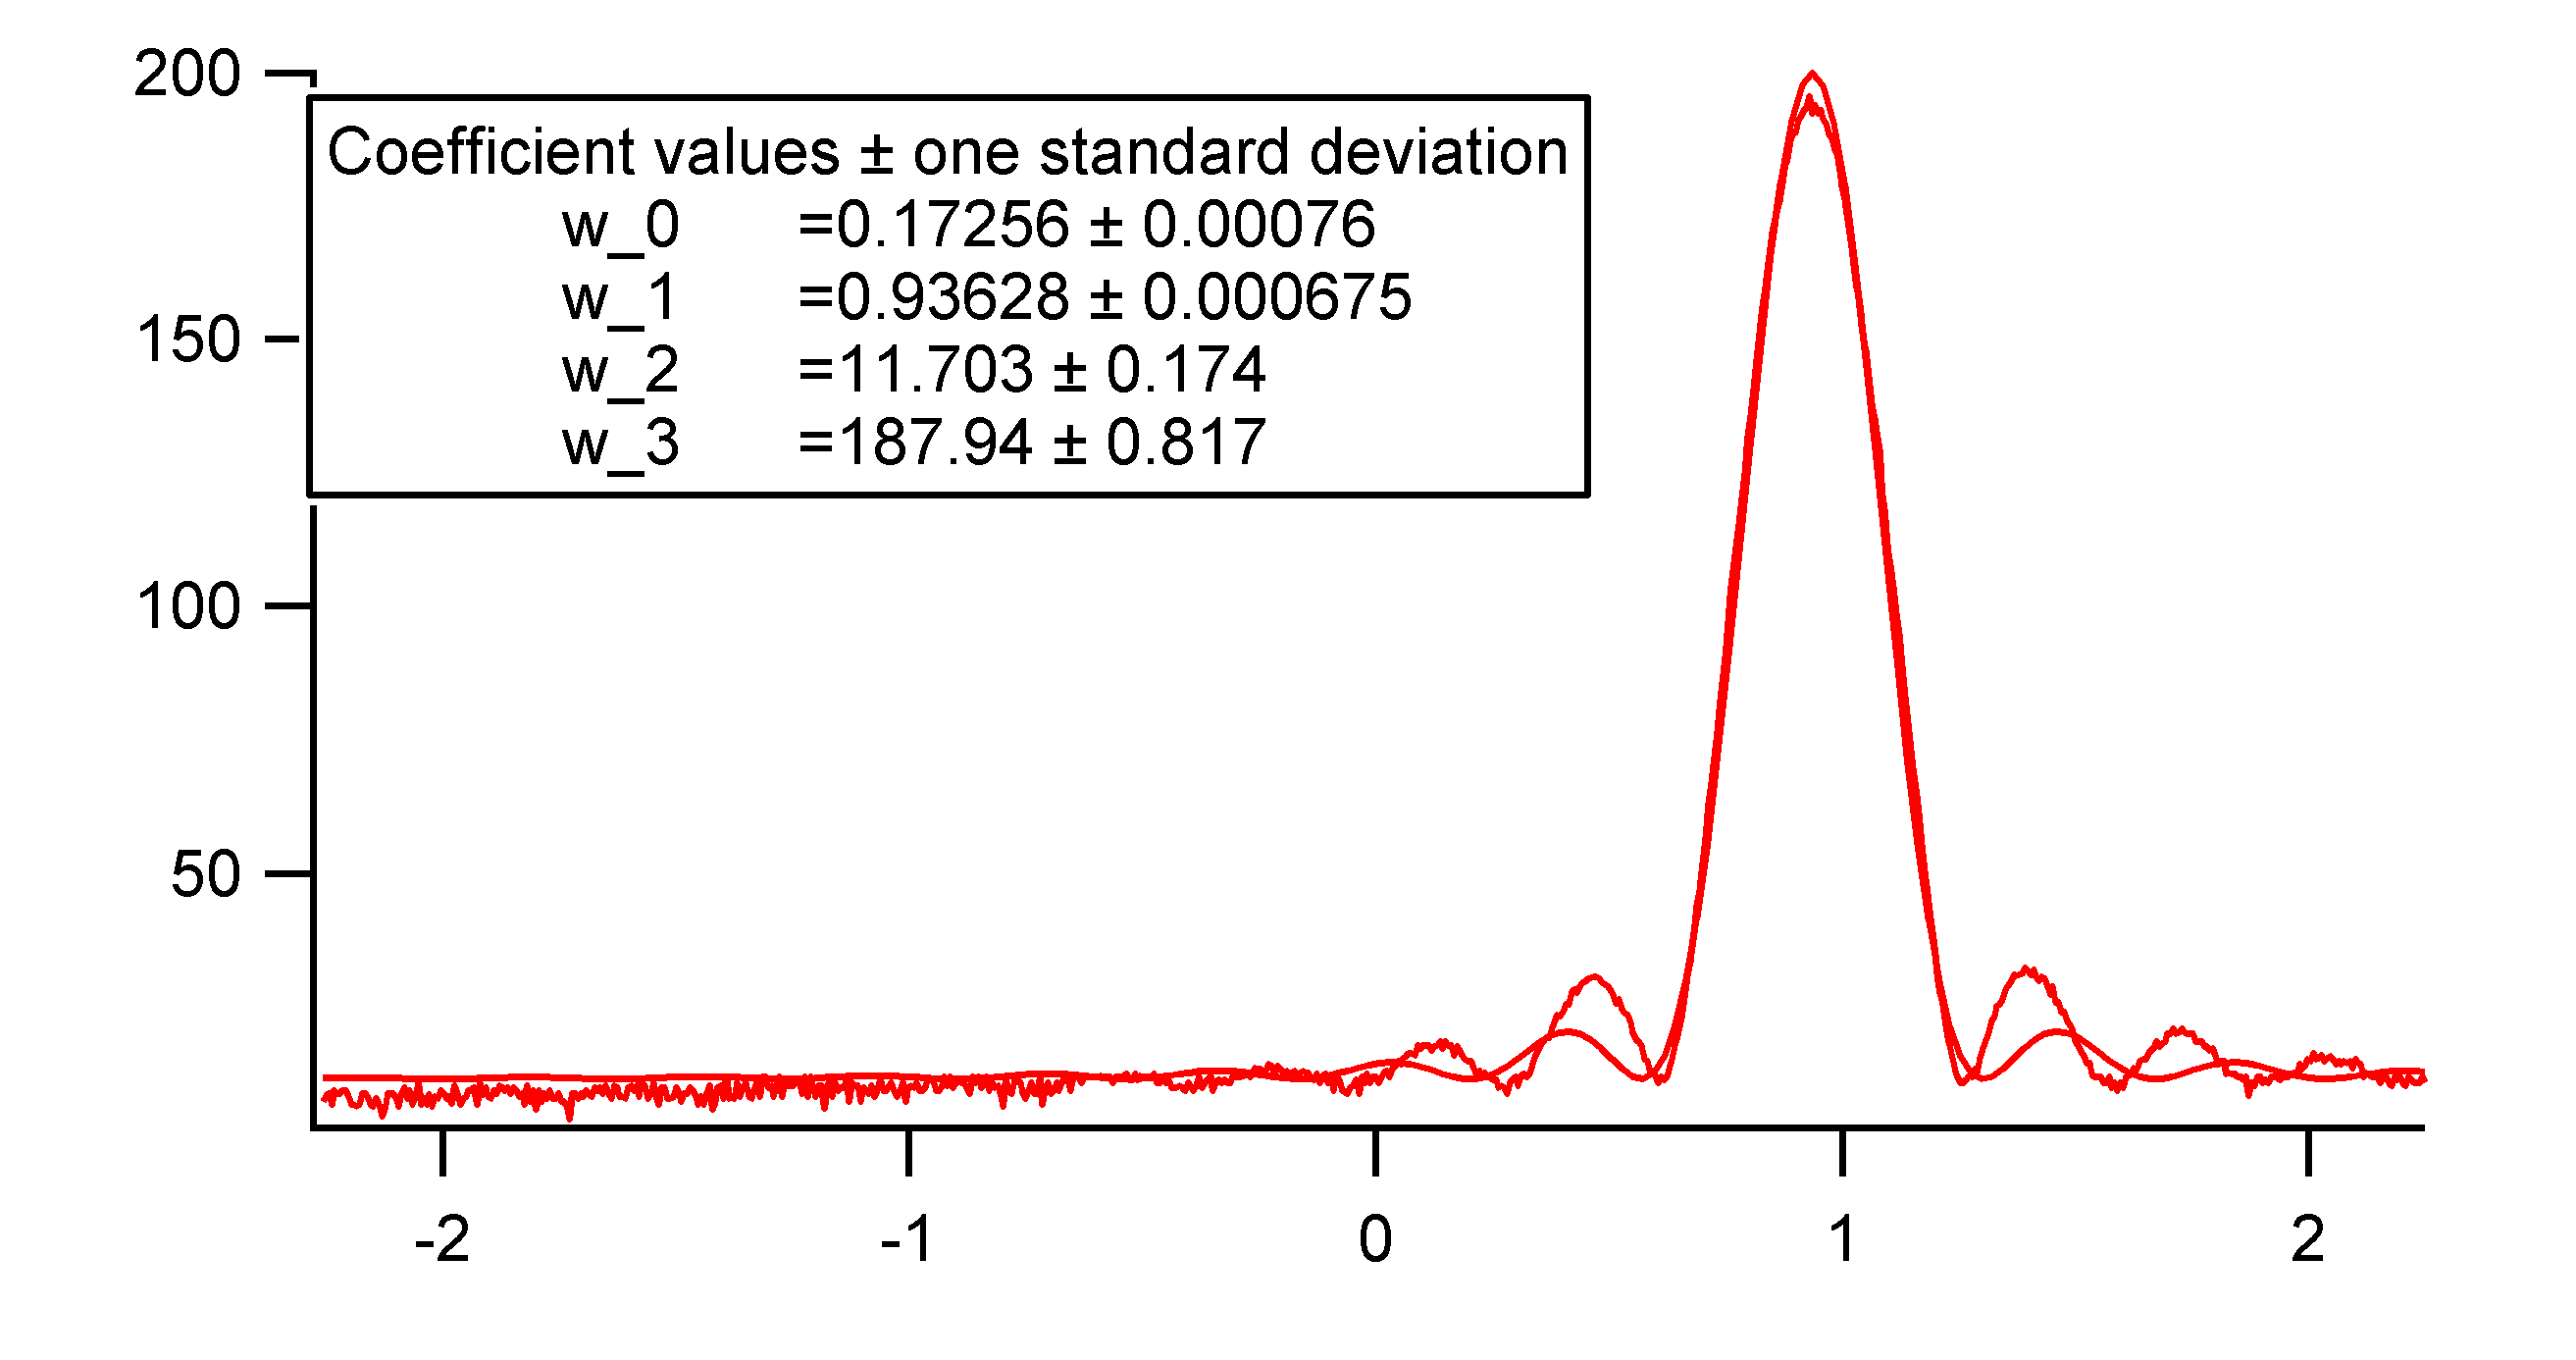
\includegraphics[width=\columnwidth]{180618/GraphSB0.png}
	\end{minipage}
	\caption{Intensitätsprofil eines Helium-Neon-Lasers bei der Einstellung von $0$. Das Profil wurde mit Igor Pro gefittet um die tatsächliche Spaltbreite exakt zu bestimmen }
	\label{HeNe_0_Prof}
\end{figure}

Durch die oben gezeigte Messung bei einer Einstellung von $0$, $4$, $8$, $12$, $16$, $20$ und $24$ konnte eine Kallibriergerade erstellt werden, bei der die Spaltbreite gegen die Einstellung des Spaltes aufgetragen wurde.

\begin{figure}[H]
	\centering	
	\begin{minipage}{1\textwidth}
		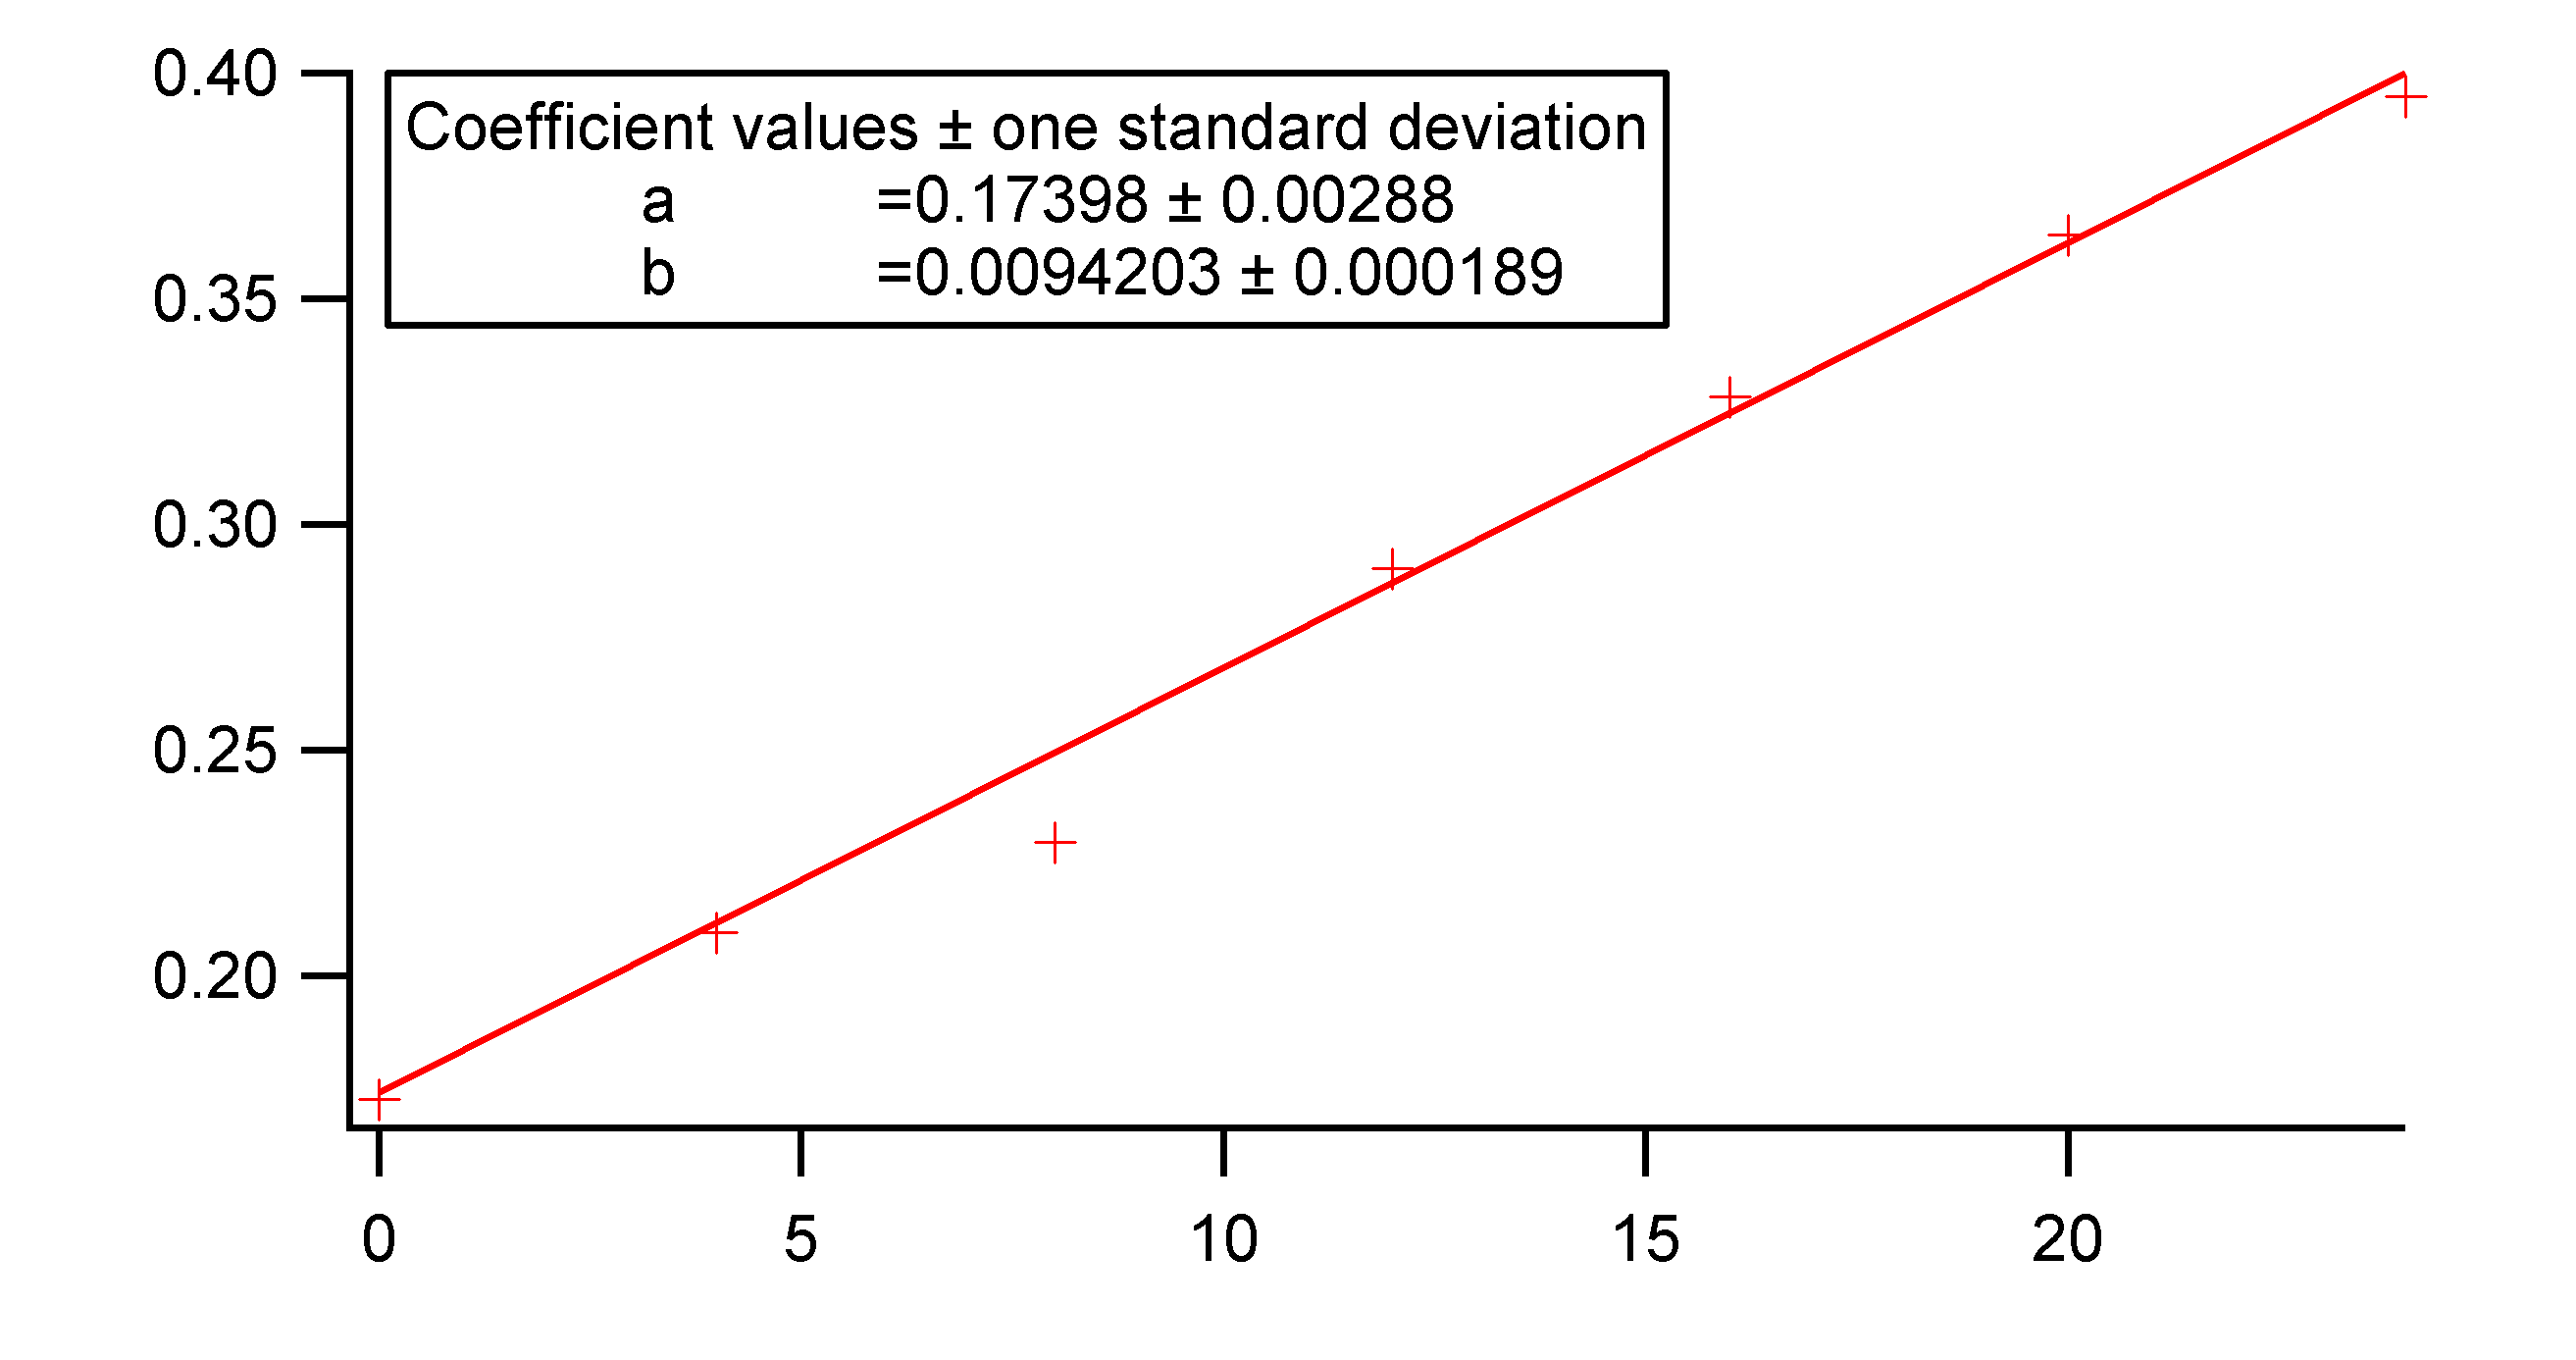
\includegraphics[width=\columnwidth]{180618/Graph_kal.png}
	\end{minipage}
	\caption{Auftragung der gemessenen Spaltbreite gegen die Einstellung am Spalt mit einer linearen Regression, dargestellt mit Igor Pro. Das Wertepaar für die Spalteinstellung von $8$ wurde bei der Regression nicht berücksichtigt, da er sichtlich von dem Trend abweicht.}
	\label{HeNe_0_Prof}
\end{figure}

Durch die exakte Bestimmung der Spaltbreite bei einer Einstellung war es nun möglich die Wellenlänge unbekannter Laser zu  ermitteln. Hierzu wurden erneut die Beugungsmuster und dadurch die Intensitätsprofile bei einer Spalteinstellung von $8~\mu m$ gemessen und aus einem Fit die Wellenlänge zu bestimmen. Die Spalteinstellung von $8$ wurde aus dem Grund gewählt, da hier die gemessene Spaltöffnung rund $250~\mu m$ betrug. Bei größenen Spaltbreiten würde der Detektor überladen, bei kleineren hingegen zu wenig anzeigen.

 Die Intensitätsprofile eines roten \ref{U_Rot}, blauen \ref{U_Blau} und eines infraroten Lasers \ref{U_IR} sind unten dargestellt. $w_0$ entsprcht hierbei der Wellenlänge. 

\begin{figure}[H]
	\centering	
	\begin{minipage}{1\textwidth}
		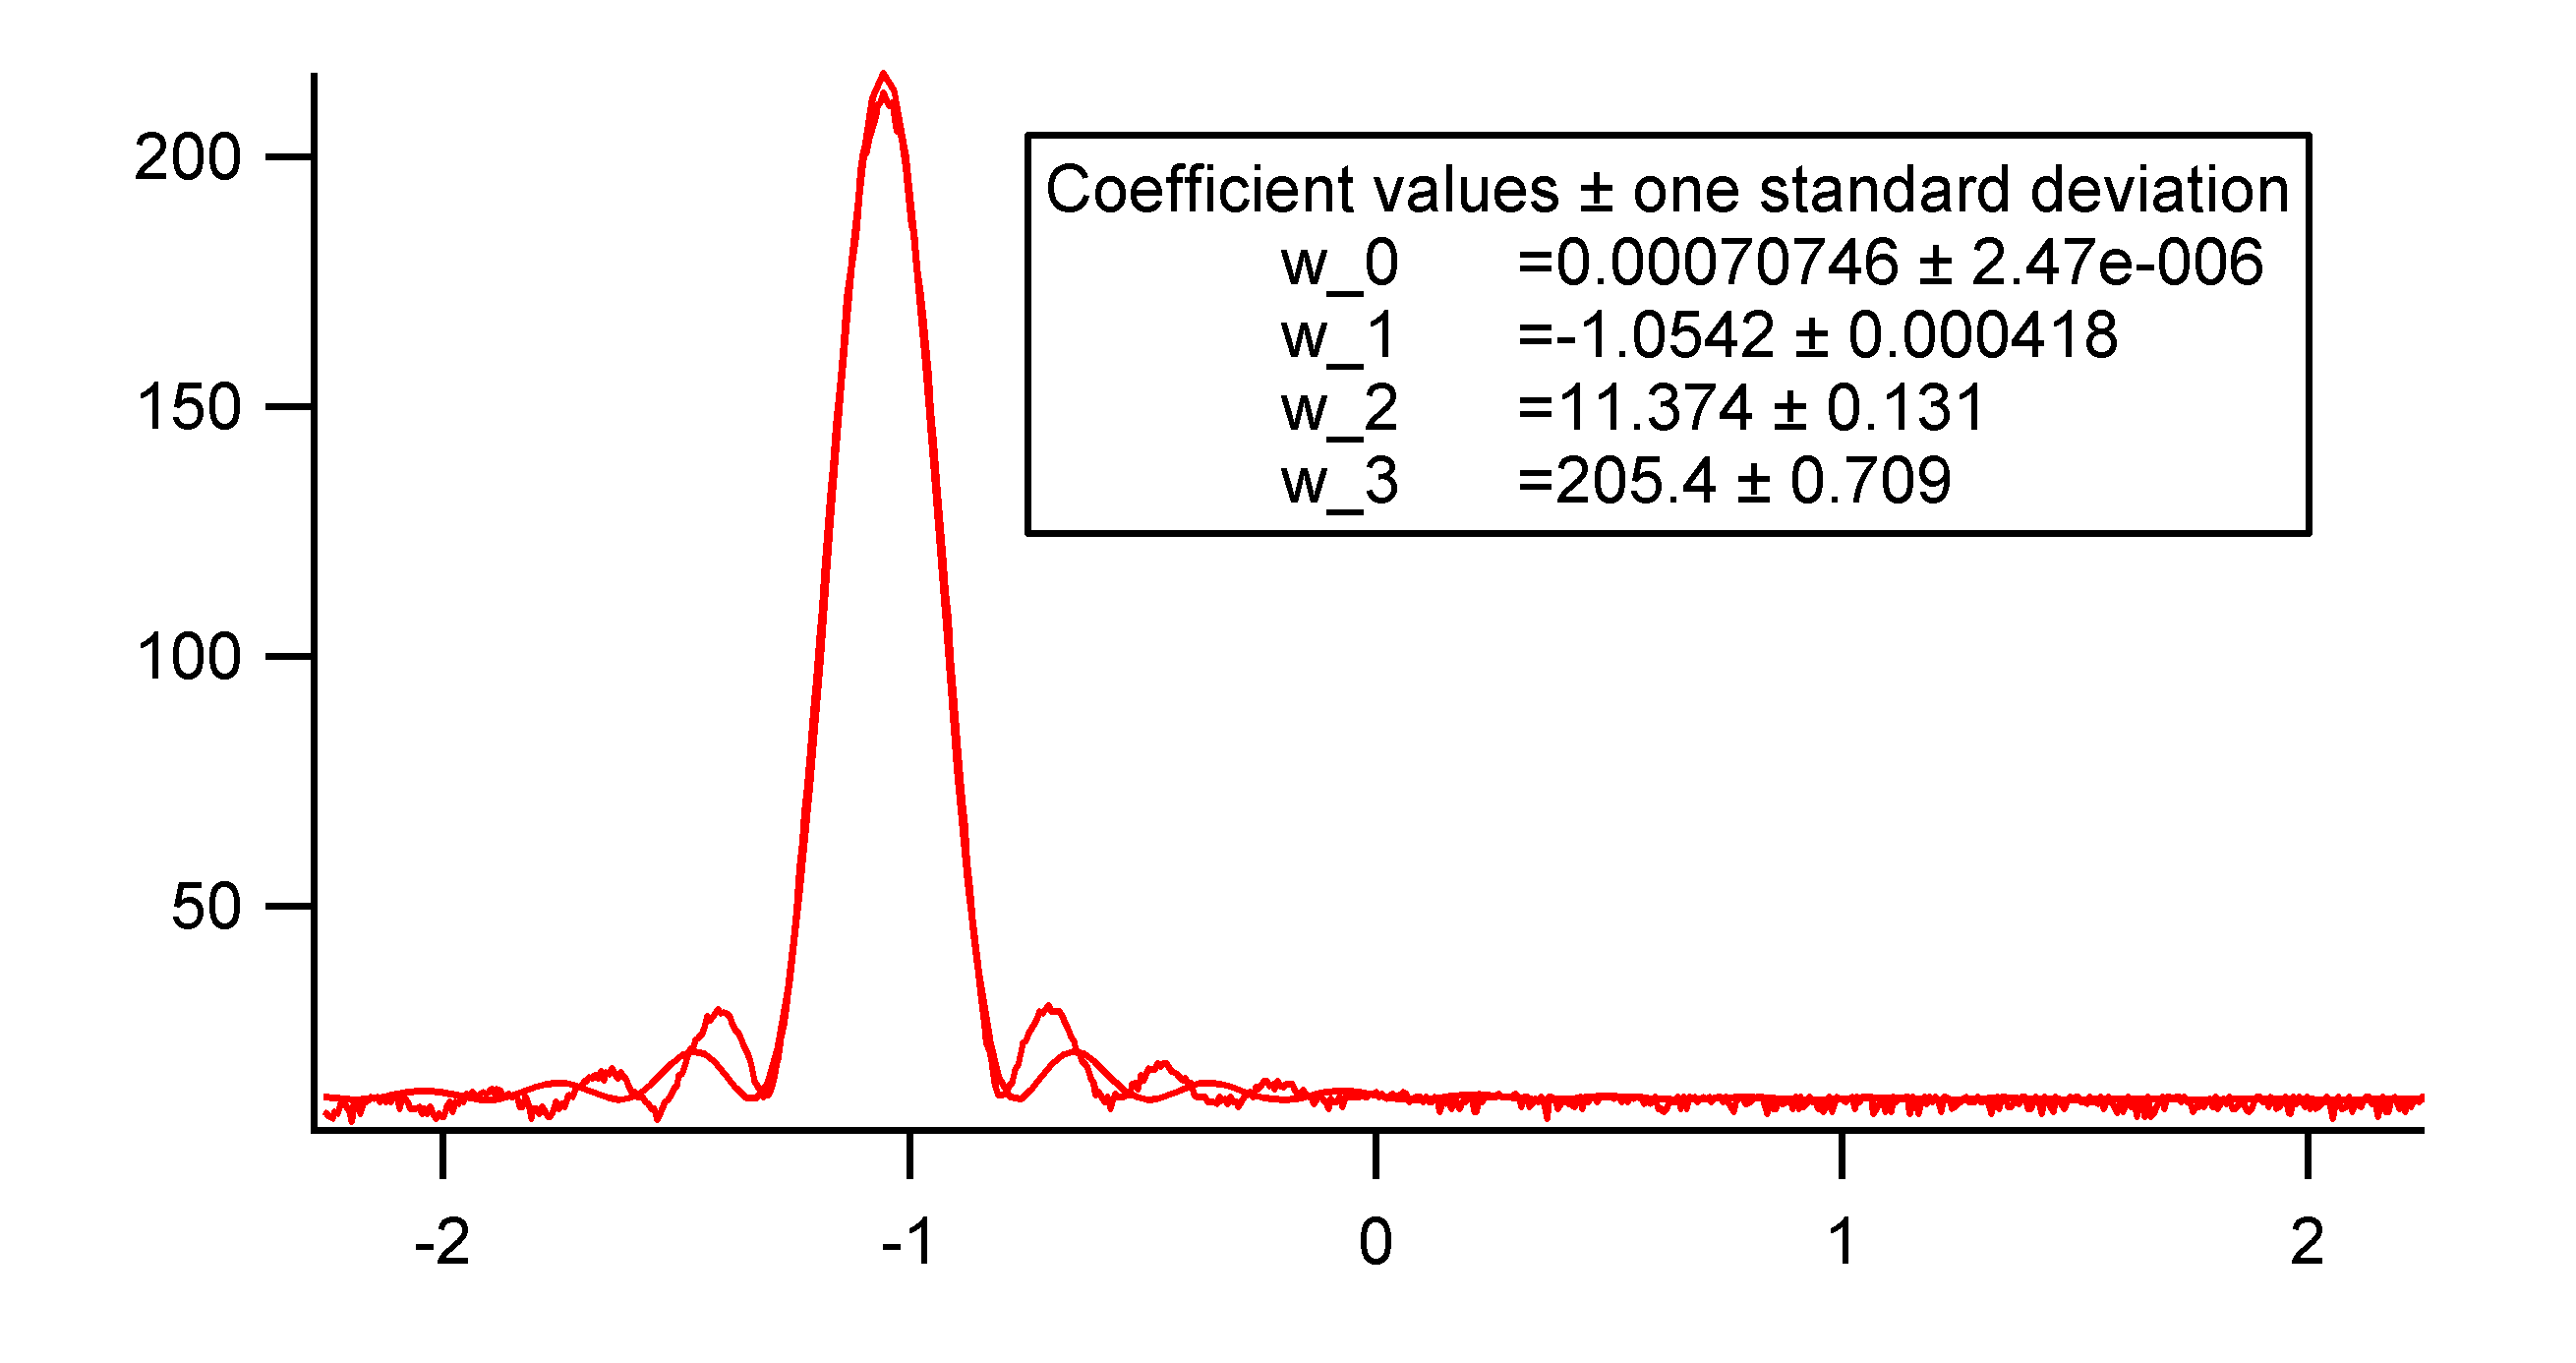
\includegraphics[width=\columnwidth]{180618/Graph_Rot.png}
	\end{minipage}
	\caption{Intensitätsprofil eines unbekannten roten Lasers bei der Einstellung von $8$. Das Profil wurde mit Igor Pro gefittet um die Wellenlänge zu ermitteln. }
	\label{U_Rot}
\end{figure}
\begin{figure}[H]
	\centering	
	\begin{minipage}{1\textwidth}
		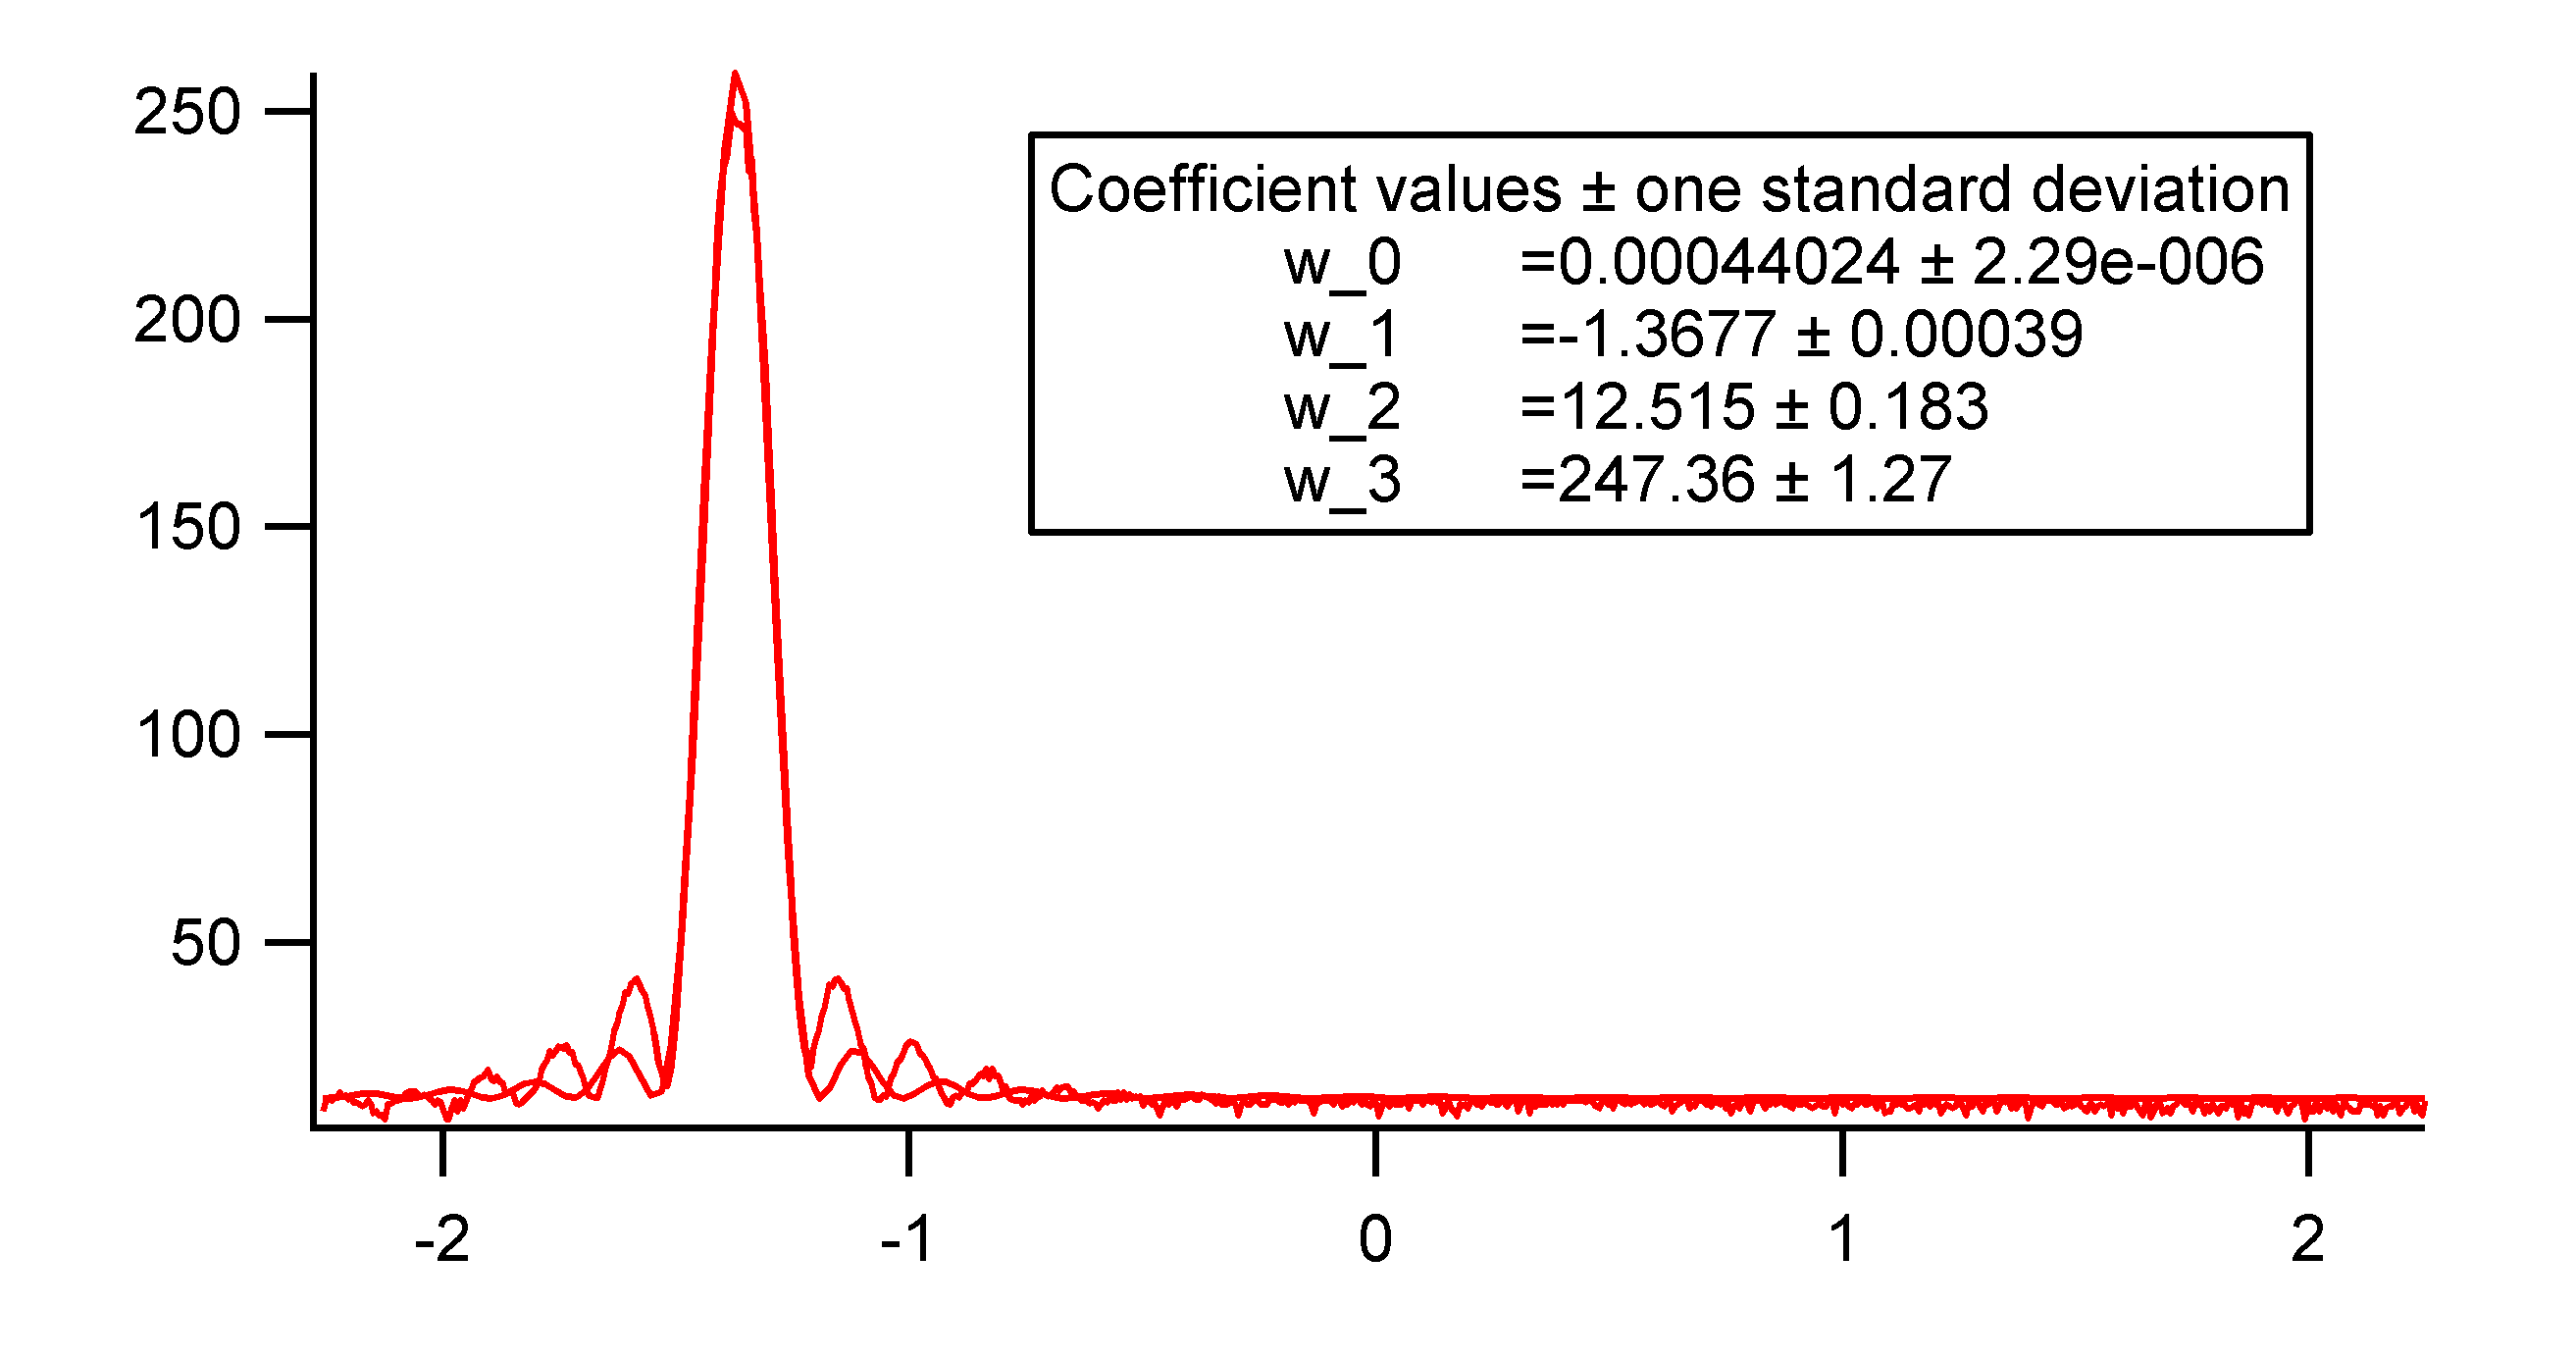
\includegraphics[width=\columnwidth]{180618/Graph_Blau.png}
	\end{minipage}
	\caption{Intensitätsprofil eines unbekannten blauen Lasers bei der Einstellung von $8$. Das Profil wurde mit Igor Pro gefittet um die Wellenlänge zu ermitteln. }
	\label{U_Blau}
\end{figure}
\begin{figure}[H]	\centering	
	\begin{minipage}{1\textwidth}
		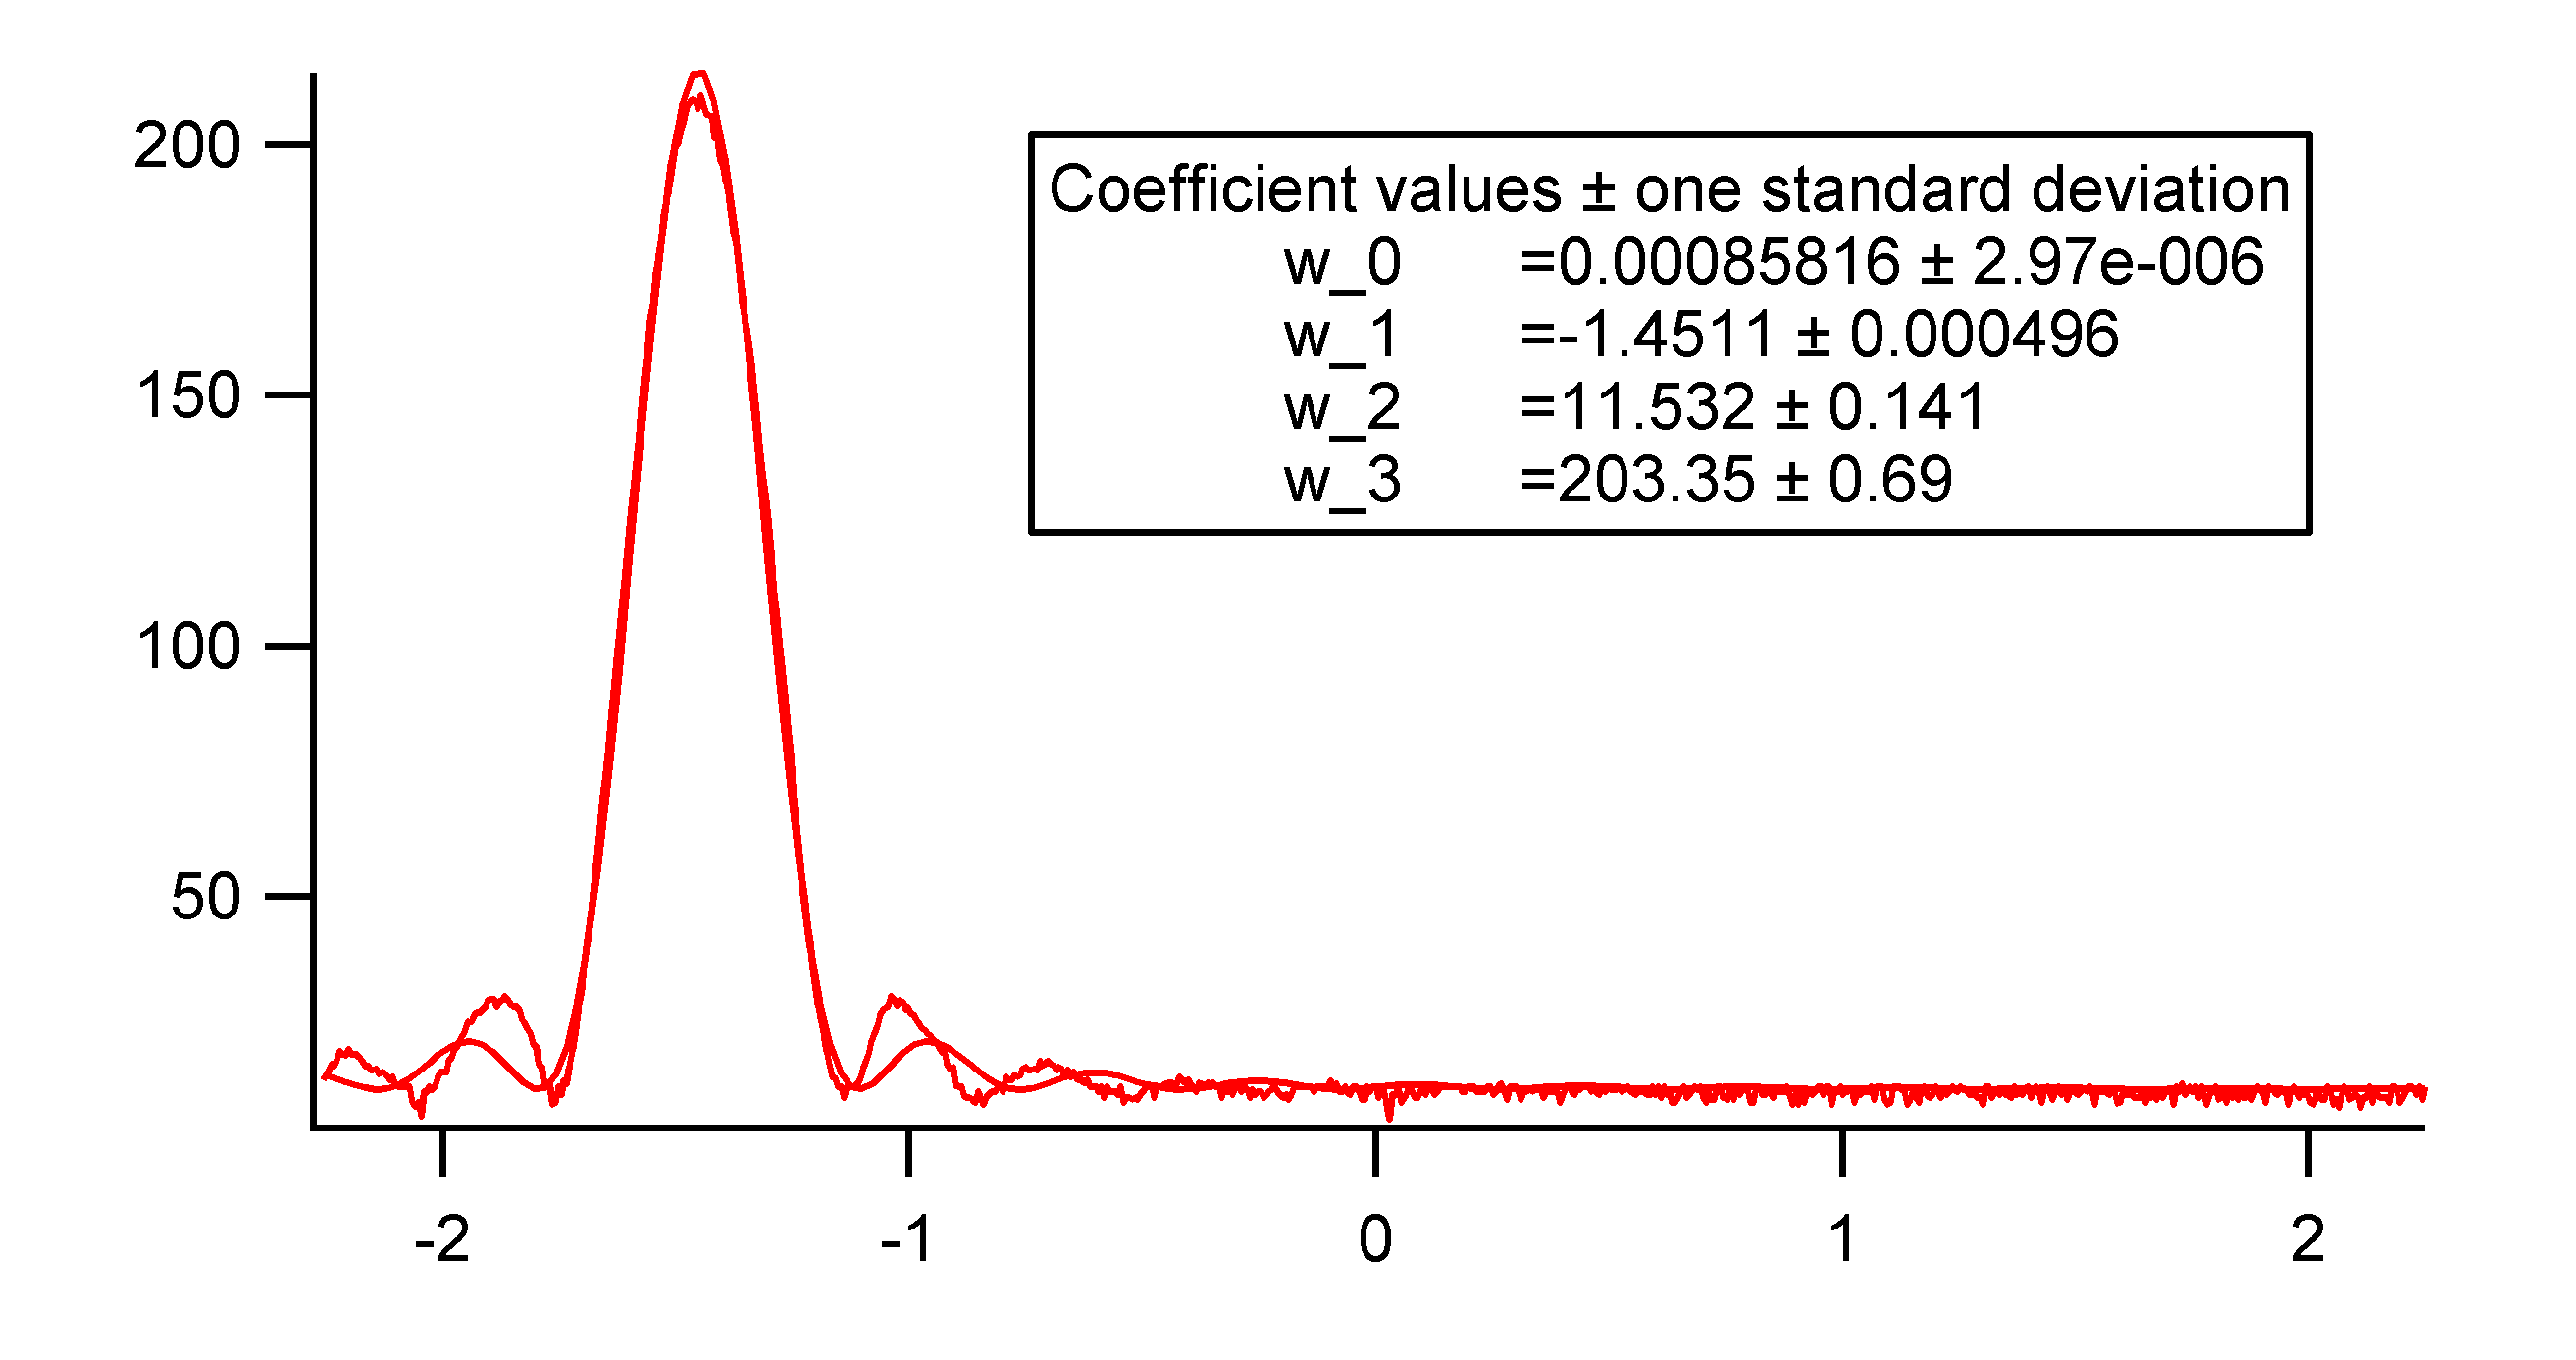
\includegraphics[width=\columnwidth]{180618/Graph_IR.png}
	\end{minipage}
	\caption{Intensitätsprofil eines unbekannten infraroten Lasers bei der Einstellung von $8$. Das Profil wurde mit Igor Pro gefittet um die Wellenlänge zu ermitteln. }
	\label{U_IR}
\end{figure}
Die Wellenlängen der unbekannten Laser wurden in Tabelle \ref{Zusammenfassung} zusammengefasst.
\begin{table}[H]
\centering

	\caption{Zusammenfassung der ermittelten Wellenlängen der unbekannten Laser }
	\begin{tabular}{C{0.15\linewidth}|C{0.15\linewidth}|C{0.15\linewidth}}
		Laser & Wellenlänge in nm & Literaturwert in nm\\
		\hline \addlinespace[1ex] 
		$ rot $ & $707.5 \pm 21.2 $ & $630 - 750$\\
		$ blau $ & $440.2 \pm 13.0$ & $ 430 - 480$\\
		$ infrarot $ & $858.2 \pm 25.7$ & $750 - 3000$ \\
\label{Zusammenfassung}	
\end{tabular}
\end{table}

Die Fehler der Wellenlängen wurden berechnet indem mit Igor Pro pro Laser zwei weitere Fits gemacht wurden. Nämlich einmal mit einem Abstand zwischen Spalt und Linse von $97~mm$ für den oberen und $103~mm$ für den unteren Wert. Der Fehler entsprcht dann dem arithmetischen Mittel der Beträge der Subtraktionen der jeweiligen Werte zum Wert bei $100~mm$. Die Fehlerbrechnung beschränkt sich auf den Fehler des Abstandes von Spalt und Linse, da dies die größte Fehlerquelle ist. 

Die gemessenen Wellenlängen liegen in den Bereichen der jeweiligen Farben. Der blaue Laser ist jedoch an der unteren Grenze des Bereichs. Dies passt jedoch gut zu der Farberscheinung des Lasers, die vom Bläulichen eher ins Violette ging und eher schwach zu sehen war, dies deutet auf eine eher kürzere Wellenlänge, als ein normaler Blauer Laser vermuten lässt hin.

%\end{document}